\chapter{परिक्षेपण और तरंग-पुंज}\label{ch:b2:dispersion-wave-packets}

तालाब में पत्थर गिराइए और तरंगिकाओं का छल्ला देखिए: नए शिखर उसके भीतरी
किनारे पर जन्मते हैं, छल्ले में से होकर बाहर दौड़ते हैं, और उसके बाहरी
किनारे पर मर जाते हैं --- अर्थात् पूरा छल्ला अपने शिखरों से धीमे चलता है।
किसी दूर के तूफ़ान के बाद समुद्र-तट पर बैठिए और लंबी, धीमी स्वेल छोटी
लहरों से एक दिन पहले आ पहुँचती है: समुद्र तरंगों को तरंगदैर्घ्य से छाँट
देता है। 1858 की पहली अटलांटिक-पार तार-केबल तड़ाकदार बिंदुओं और रेखाओं
को ऐसी लीप में बदल देती थी जिसे पढ़ने में मिनट लगते। तीनों दशाओं में
तरंग की चाल उसकी आवृत्ति पर निर्भर है: अर्थात् माध्यम
\emph{परिक्षेपी} है। यह अध्याय \omterm{def:b2:dispersion-wave-packets:relation}{परिक्षेपण संबंध}, वह
\omterm{def:b2:dispersion-wave-packets:complex}{सम्मिश्र तरंग-संख्या} जो संचरण और अवशोषण दोनों ढोती है, वह \omterm{prop:b2:dispersion-wave-packets:group}{समूह वेग}
जिससे कोई पुंज --- और उसकी ऊर्जा, और उसकी सूचना --- वास्तव में चलती है, और
वह रेखा प्रस्तुत करता है जिसके अनुदिश तार-संचार, दूरदर्शन और
इंटरनेट चले हैं: अर्थात् \omterm{prop:b2:dispersion-wave-packets:coax}{समाक्ष केबल}।

\section{परिक्षेपण संबंध}

\begin{definition}[परिक्षेपण संबंध; कला वेग]\label{def:b2:dispersion-wave-packets:relation}
\index{परिक्षेपण संबंध}\index{कला वेग}\index{परिक्षेपी माध्यम}
कोई रैखिक, समांगी, समय-अपरिवर्ती माध्यम समतल
एकवर्णी तरंगें $\underline s = A\,\eu^{\iu(\omega t - kx)}$ स्वीकार करता है (सम्मिश्र
संकेतन; भौतिक संकेत वास्तविक भाग है), बशर्ते $\omega$ और $k$
माध्यम के \emph{परिक्षेपण संबंध} $\mathcal D(\omega, k)
= 0$ का पालन करें, जिसे $k(\omega)$ या $\omega(k)$ के रूप में हल किया जाता है। वास्तविक $k$ के लिए तरंग
बिना विरूपण के \emph{कला वेग} से चलती है:
\[
v_\varphi = \frac\omega k .
\]
माध्यम \emph{अपरिक्षेपी} तब कहलाता है जब $v_\varphi$
$\omega$ पर निर्भर न करे (तब $\omega = ck$ और हर संकेत बिना विरूपण संचरित होता है ---
यही \omterm{thm:b2:waves-on-strings:equation}{दालांबेर समीकरण} है), और अन्यथा \emph{परिक्षेपी}।
\end{definition}

\begin{proof}
अचर गुणांकों वाले किसी रैखिक समीकरण में $\eu^{\iu(\omega t - kx)}$ रखने पर
हर $\partial_t$ $\iu\omega$ में और हर $\partial_x$
$-\iu k$ में बदल जाता है, और पीछे एक बीजीय संबंध बचता है। तार, ध्वनि-तरंग और
छड़ ने $\omega^2 = c^2k^2$ दिया था।
\end{proof}

\begin{example}[परिक्षेपी और अपरिक्षेपी]\label{ex:b2:dispersion-wave-packets:examples}
\index{क्लाइन--गॉर्डन समीकरण}\index{गहरे पानी की तरंगें}
(क) प्रत्यास्थ शय्या पर रखा कोई तार (प्रति एकांक लंबाई प्रत्यानयन बल $-Ky$,
या लोलकों की कोई शृंखला), $\mu\partial_t^2y = T\partial_x^2y - Ky$: $\omega^2 = \omega_c^2
+ c^2k^2$, जहाँ $\omega_c = \sqrt{K/\mu}$ --- यही \emph{क्लाइन--गॉर्डन}
संबंध है, जो प्लाज़्मा और तरंग-नलिका का भी है
(\cref{ch:b2:waves-in-media,ch:b2:guided-waves}): $v_\varphi = c/\sqrt{1 -
\omega_c^2/\omega^2} > c$, और कोई वास्तविक $k$ \emph{कटाव} $\omega_c$ से नीचे नहीं।
(ख) गहरे पानी की गुरुत्व-तरंगें: $\omega^2 = gk$ (स्वीकृत), $v_\varphi =
\sqrt{g/k} = \sqrt{g\lambda/2\pi}$: अर्थात् लंबी तरंगें तेज़ --- \qty{100}{m} के लिए \qty{12.5}{m/s},
\qty{1}{km} के लिए \qty{40}{m/s}। (ग) \omterm{prop:b2:waves-on-strings:chain}{परमाणुओं की शृंखला}, $\omega =
2\omega_0|\sin(ka/2)|$ (\cref{ch:b2:waves-on-strings})। (घ) काँच में प्रकाश,
$k = n(\omega)\omega/c$, और इसीलिए कोई प्रिज़्म वर्णक्रम फैला देता है।
\end{example}

\begin{omfigure}
\begin{tikzpicture}
\begin{axis}[omaxis, axis x line=bottom, axis y line=left, width=6.2cm, height=4.6cm,
    xlabel={$k$}, ylabel={$\omega$}, xmin=0, xmax=3, ymin=0, ymax=3.3, xtick=\empty, ytick={1}, yticklabels={$\omega_c$}, samples=80,
    xlabel style={at={(axis description cs:1.0,0.0)}, anchor=west},
    ylabel style={at={(axis description cs:0.0,1.0)}, anchor=south},
    legend style={font=\scriptsize, at={(0.03,0.97)}, anchor=north west, draw=none, fill=none}]
  \addplot[omDef, thick, domain=0:3] {x};
  \addplot[omThm, thick, domain=0:3] {sqrt(1+x*x)};
  \addplot[omProp, thick, domain=0:3] {1.6*sqrt(x)};
  \legend{$\omega = ck$, $\omega^2 = \omega_c^2 + c^2k^2$, $\omega^2 = gk$}
\end{axis}
\end{tikzpicture}
\hfill
\begin{tikzpicture}
\begin{axis}[omaxis, axis x line=bottom, axis y line=left, width=6.2cm, height=4.6cm,
    xlabel={$\omega/\omega_c$}, ylabel={$v/c$}, xmin=0, xmax=4, ymin=0, ymax=2.6, xtick={1,2,3}, ytick={1}, samples=100,
    xlabel style={at={(axis description cs:0.5,-0.12)}, anchor=north},
    ylabel style={at={(axis description cs:-0.1,0.5)}, rotate=90, anchor=south},
    legend style={font=\scriptsize, at={(0.97,0.95)}, anchor=north east, draw=none, fill=none}]
  \addplot[omThm, thick, domain=1.08:4] {1/sqrt(1-1/(x*x))};
  \addplot[omDef, thick, domain=1.0:4] {sqrt(1-1/(x*x))};
  \addplot[black, dashed, domain=0:4] {1};
  \legend{$v_\varphi$, $v_g$}
  \node[font=\scriptsize, anchor=west, align=left] at (axis cs:0.05,1.9) {संचरण\\नहीं};
\end{axis}
\end{tikzpicture}

{\small बाएँ: तीन \omterm{def:b2:dispersion-wave-packets:relation}{परिक्षेपण संबंध} --- अपरिक्षेपी माध्यम के लिए सरल
रेखा, अपने कटाव के साथ क्लाइन--गॉर्डन अतिपरवलय,
और गहरे पानी की तरंगों का परवलय। दाएँ: क्लाइन--गॉर्डन
संबंध के लिए \omterm{def:b2:dispersion-wave-packets:relation}{कला वेग} $c$ से ऊपर रहता है और \omterm{prop:b2:dispersion-wave-packets:group}{समूह वेग} उससे
नीचे, तथा $v_\varphi v_g = c^2$।}
\end{omfigure}

\begin{definition}[सम्मिश्र तरंग-संख्या: संचरण और क्षीणन]\label{def:b2:dispersion-wave-packets:complex}
\index{सम्मिश्र तरंग-संख्या}\index{क्षीणन}\index{क्षयी तरंग}\index{त्वचा गहराई}
जब \omterm{def:b2:dispersion-wave-packets:relation}{परिक्षेपण संबंध} वास्तविक $\omega$ के लिए कोई सम्मिश्र
$\underline k = k' - \iu k''$ देता है, तब तरंग
\[
\underline s = A\,\eu^{-k''x}\,\eu^{\iu(\omega t - k'x)} :
\]
होती है: वह $v_\varphi = \omega/k'$ से संचरित होती है और उसका आयाम
$\eu^{-x/\delta}$ की तरह क्षय होता है, जहाँ \emph{क्षीणन लंबाई} $\delta = 1/k''$ है (उसे
अपनी संचरण-दिशा में क्षय होना चाहिए: अतः $k'$ और $k''$ एक ही चिह्न के)।
यदि $\underline k$ शुद्ध काल्पनिक हो, $\underline k = -\iu\kappa$, तो तरंग
\emph{क्षयी} है: $A\,\eu^{-\kappa x}\eu^{\iu\omega t}$, अर्थात् कोई अप्रगामी दोलन
जिसका आयाम $1/\kappa$ दूरी में मर जाता है और जो कुछ भी संचरित नहीं करता
--- यही अपने कटाव से नीचे क्लाइन--गॉर्डन माध्यम की दशा है,
$\kappa = \sqrt{\omega_c^2 - \omega^2}/c$, और प्रकाशिक आवृत्तियों पर किसी धातु की।
\end{definition}

\begin{example}[अवमंदित तार]\label{ex:b2:dispersion-wave-packets:damped}
किसी श्यान तरल में तार, $\mu\partial_t^2y + \alpha\partial_ty = T\partial_x^2y$:
$\underline k^2 = (\omega^2 - \iu\alpha\omega/\mu)/c^2$। दुर्बल अवमंदन ($\alpha \ll \mu
\omega$) के लिए $\underline k \approx \dfrac\omega c\Bigl(1 - \iu\dfrac{\alpha}{2\mu\omega}\Bigr)$: अर्थात् तरंग
अपनी चाल बनाए रखती है और $\delta = 2\mu c/\alpha = 2Z/\alpha$ में आयाम खोती है,
और वह भी आवृत्ति से स्वतंत्र --- अर्थात् कोई \emph{क्षयकारी}, अपरिक्षेपी हानि,
प्रति $\delta$ लंबाई \qty{8.7}{dB}।
\end{example}

\section{तरंग-पुंज और समूह वेग}

\begin{proposition}[विस्पंद; समूह वेग]\label{prop:b2:dispersion-wave-packets:group}
\index{समूह वेग}\index{तरंग-पुंज}\index{विस्पंद}
बराबर आयाम और पड़ोसी आवृत्तियों $\omega \pm
\delta\omega$ तथा तरंग-संख्याओं $k \pm \delta k$ की दो तरंगें अध्यारोपित होकर बनती हैं:
\[
s = 2A\cos(\delta\omega\,t - \delta k\,x)\cos(\omega t - kx) :
\]
अर्थात् $(\omega, k)$ पर कोई वाहक, जो $v_\varphi = \omega/k$ से चलता है, और उस पर
किसी धीमे आवरण का मॉडुलन, जो $\delta\omega/\delta k$ से चलता है। कोई \emph{\omterm{prop:b2:dispersion-wave-packets:group}{तरंग-पुंज}} ---
अर्थात् $k_0$ के चारों ओर सँकरी पट्टी की तरंग-संख्याओं वाली एकवर्णी तरंगों का
अध्यारोपण --- समग्र रूप से \emph{\omterm{prop:b2:dispersion-wave-packets:group}{समूह वेग}} से चलता है:
\[
v_g = \frac{\dd\omega}{\dd k}\Bigr|_{k_0} ,
\]
और यही उसकी ऊर्जा का तथा उसकी ढोई गई सूचना का वेग है।
अपरिक्षेपी माध्यम में $v_g = v_\varphi = c$; अन्यथा पुंज चलते-चलते
विरूपित होता है (वह \emph{फैलता} है), और $\dd^2\omega/\dd k^2$ जितना बड़ा तथा
उसके वर्णक्रम की पूरक राशि, अर्थात् उसकी आकाशी चौड़ाई, जितनी सँकरी, उतना
ही तेज़।
\end{proposition}

\begin{proof}
योग-से-गुणनफल का सूत्र विस्पंद देता है। किसी पुंज के लिए $s =
\int a(k)\eu^{\iu(\omega(k)t - kx)}\dd k$ लिखिए (एक फूरिये अध्यारोपण ---
फूरिये समाकल वर्ष 3 के गणित-खंड में पढ़ा जाता है; यहाँ केवल
उसका ज्यावक्रों के सतत योग वाला अर्थ काम में आता है), जहाँ
$a(k)$ का शिखर $k_0$ पर हो। अब $\omega(k) \approx \omega_0 + v_g(k - k_0)$ को फैलाइए: तब
$s \approx \eu^{\iu(\omega_0t - k_0x)}\int a(k)\eu^{\iu(k - k_0)(v_gt - x)}\dd k$ मिलता है, अर्थात् कोई
वाहक गुणा कोई ऐसा आवरण जो केवल $x - v_gt$ का फलन है --- अतः
आवरण $v_g$ से चलता है। अगला पद, $\tfrac12\omega''(k_0)(k - k_0)^2t$,
घटकों की कला समय में बिगाड़ देता है और आवरण को फैला देता है। किसी पुंज की
ऊर्जा वहीं होती है जहाँ उसका आवरण; और कोई भी संकेत भी वहीं।
\end{proof}

\begin{omfigure}
\begin{tikzpicture}
\begin{axis}[omaxis, axis x line=middle, axis y line=none, width=13.6cm, height=4.0cm,
    xmin=0, xmax=60, ymin=-3.1, ymax=3.3, xtick=\empty, samples=600, xlabel={$x$}, clip=false,
    xlabel style={at={(axis description cs:1.0,0.5)}, anchor=west}]
  \addplot[omDef, thick, domain=0:60] {2*cos(deg(0.12*x))*cos(deg(2.2*x))};
  \addplot[omThm, thick, domain=0:60] {2*cos(deg(0.12*x))};
  \addplot[omThm, thick, domain=0:60] {-2*cos(deg(0.12*x))};
  \draw[omThm, very thick, ->] (axis cs:9,2.6) -- (axis cs:15,2.6) node[above, font=\scriptsize, pos=0.5] {$v_g$};
  \draw[omDef, very thick, ->] (axis cs:38,-2.6) -- (axis cs:48,-2.6) node[below, font=\scriptsize, pos=0.5] {$v_\varphi$};
\end{axis}
\end{tikzpicture}

{\small विस्पंद: दो पड़ोसी आवृत्तियाँ कोई तेज़ वाहक बनाती हैं
(जो \omterm{def:b2:dispersion-wave-packets:relation}{कला वेग} से चलता है) और उस पर कोई धीमा आवरण (जो \omterm{prop:b2:dispersion-wave-packets:group}{समूह
वेग} से चलता है); और \omterm{def:b2:dispersion-wave-packets:relation}{परिक्षेपी माध्यम} में दोनों चालें भिन्न होती हैं तथा
शिखर आवरण में से होकर सरकते जाते हैं।}
\end{omfigure}

\begin{example}[गहरा पानी: शिखर समूह से आगे निकल जाते हैं]\label{ex:b2:dispersion-wave-packets:deepwater}
$\omega = \sqrt{gk}$: अतः $v_g = \tfrac12\sqrt{g/k} = \tfrac12v_\varphi$। स्वेल का कोई
समूह अपने शिखरों से आधी चाल से चलता है: किसी तरंग-रेल को देखते हुए
आप शिखरों को समूह के पीछे उभरते, उसमें से गुज़रते और
आगे लुप्त होते देखते हैं --- ठीक वही तालाब का छल्ला। \qty{3000}{km} दूर
का कोई तूफ़ान अपनी \qty{15}{s} की स्वेल ($\lambda = gT^2/2\pi = \qty{350}{m}$, $v_g =
gT/4\pi = \qty{11.7}{m/s}$) तीन दिन में भेजता है, और अपनी \qty{8}{s} की तरंगें ($v_g =
\qty{6.2}{m/s}$) साढ़े पाँच में: अतः भिन्न आवर्तकालों के आने के समय से
समुद्र-विज्ञानी तूफ़ान की जगह ढूँढ़ लेते हैं।
\end{example}

\begin{omfigure}
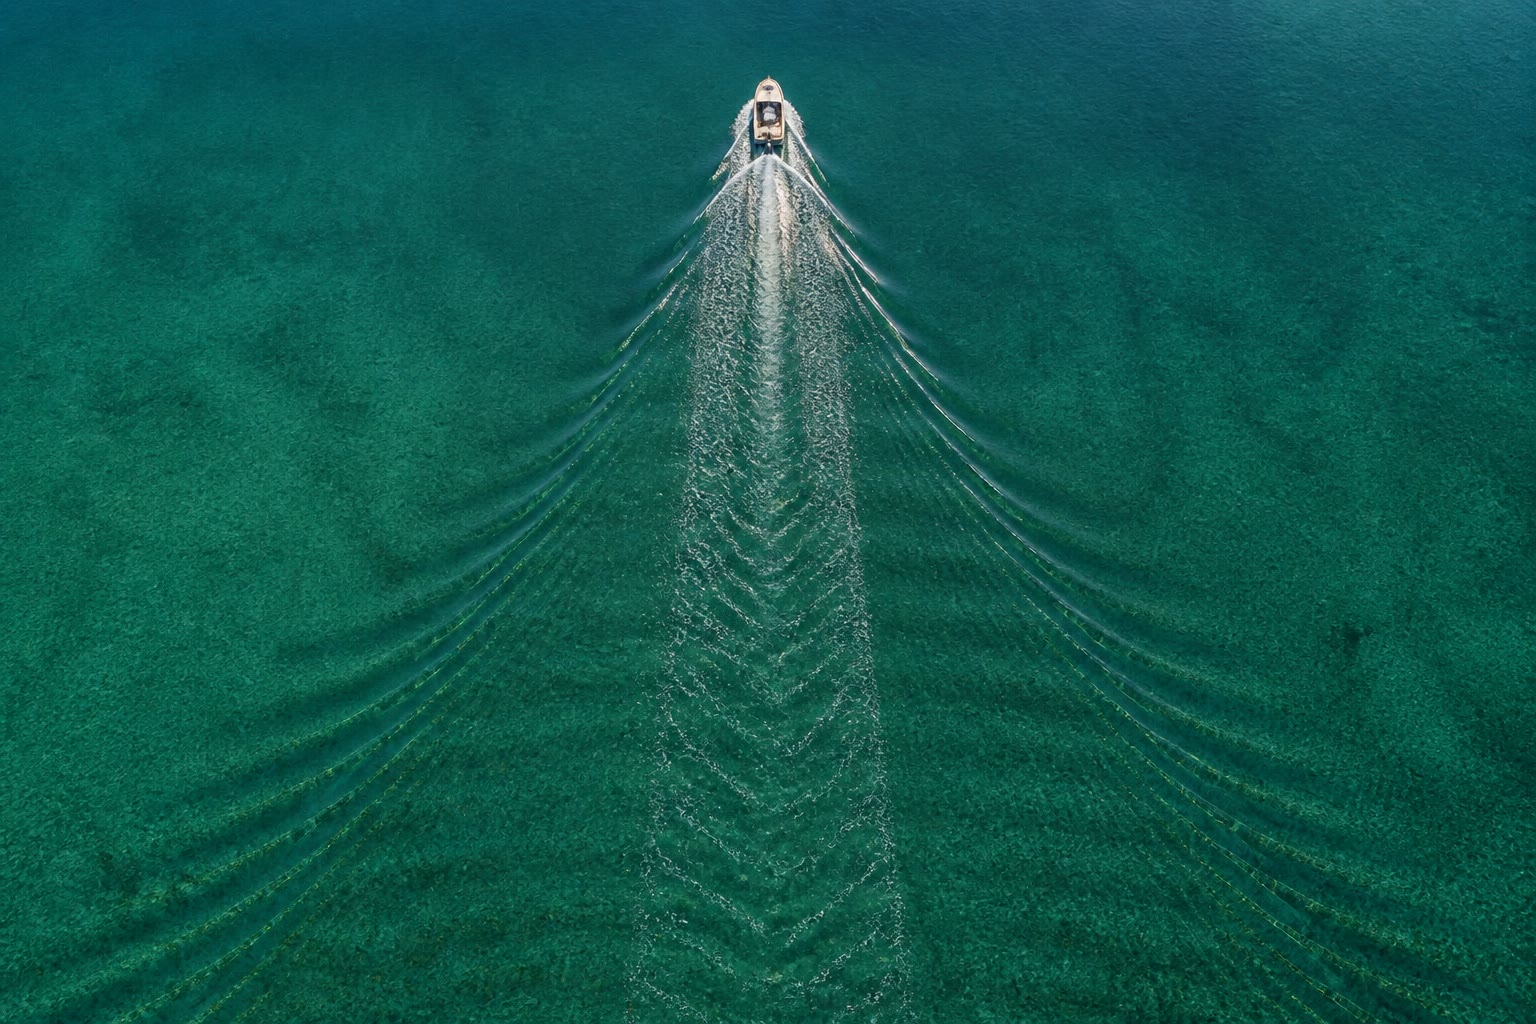
\includegraphics[width=0.56\linewidth]{images/book4/ai/b4-08-boat-wake-aerial.jpg}

{\small किसी शांत झील पर मोटरबोट का अनुतरंग: पंखनुमा आकृति नियत कोण की फाँक के भीतर बनी रहती है, क्योंकि हर जल-तरंग की ऊर्जा उसके शिखरों की आधी चाल से चलती है --- अर्थात् परिक्षेपण, आँखों देखा।}
\end{omfigure}


\begin{example}[क्लाइन--गॉर्डन: प्रकाश से तेज़, और फिर भी नहीं]\label{ex:b2:dispersion-wave-packets:superluminal}
$\omega^2 = \omega_c^2 + c^2k^2$ के लिए: $v_\varphi = \omega/k$ और $v_g = c^2k/\omega$, अतः
$v_\varphi v_g = c^2$: \omterm{def:b2:dispersion-wave-packets:relation}{कला वेग} $c$ से ऊपर रहता है (आयनमंडल में किसी
\qty{10}{MHz} तरंग के शिखर प्रकाश से तेज़ चलते हैं), पर \omterm{prop:b2:dispersion-wave-packets:group}{समूह
वेग}, जो संकेत ढोता है, उससे नीचे रहता है। \omterm{def:b2:dispersion-wave-packets:relation}{कला वेग}
न ऊर्जा ढोता है न सूचना --- शिखर उस प्रकाश-स्तंभ की धब्बे जैसे हैं जो
किसी दूर के बादल पर झाड़ू फेरती है।
\end{example}

\begin{remark}[फैलाव]\label{rem:b2:dispersion-wave-packets:spreading}
$\Delta x$ आकाशी चौड़ाई के किसी पुंज में तरंग-संख्याएँ $\Delta k \sim
1/\Delta x$ भर फैली होती हैं (फूरिये की व्युत्क्रमता, स्वीकृत); उसके घटकों के \omterm{prop:b2:dispersion-wave-packets:group}{समूह
वेग} $\Delta v_g \approx |\omega''|\Delta k$ से भिन्न होते हैं, अतः समय $t$ बाद वह
$|\omega''|\Delta k\,t$ फैल चुका होता है: और $t_{\text{फैलाव}}
\sim \Delta x^2/|\omega''|$ बाद उसकी चौड़ाई दुगुनी हो जाती है। \qty{100}{m} की दस गहरे-पानी तरंगों का पुंज
($\Delta x \approx \qty{1}{km}$, $\omega'' = -\tfrac14\sqrt{g/k^3} = \qty{-50}{m^2/s}$)
लगभग छह घंटे में दुगुना हो जाता है; और किसी प्रकाशिक तंतु में \qty{1}{ns} का
प्रकाश-स्पंद प्रति किलोमीटर दसियों पिकोसेकंड फैल जाता है --- यही लंबी
कड़ियों की बिट-दर की सीमा है। \cref{ch:b2:schrodinger-wave-functions} का
क्वांटम \omterm{prop:b2:dispersion-wave-packets:group}{तरंग-पुंज} भी इसी कारण फैलता है।
\end{remark}

\section{समाक्ष केबल}

\begin{proposition}[टेलीग्राफ समीकरण; हानि-रहित रेखा]\label{prop:b2:dispersion-wave-packets:coax}
\index{समाक्ष केबल}\index{टेलीग्राफ समीकरण}\index{अभिलक्षणिक प्रतिबाधा}\index{संचरण-रेखा}
किसी \omterm{prop:b2:dispersion-wave-packets:coax}{समाक्ष केबल} (या किसी भी दो-चालक रेखा) में प्रति एकांक लंबाई
प्रेरकत्व $\Lambda$ और धारिता $\Gamma$ होती है। चालकों के बीच वोल्टता $v(x, t)$
और भीतरी चालक में धारा $i(x, t)$ इन
\emph{\omterm{prop:b2:dispersion-wave-packets:coax}{टेलीग्राफ समीकरणों}} का पालन करती हैं:
\[
\frac{\partial v}{\partial x} = -\Lambda\frac{\partial i}{\partial t} , \qquad
\frac{\partial i}{\partial x} = -\Gamma\frac{\partial v}{\partial t} ,
\]
अतः $v$ और $i$ के लिए \omterm{thm:b2:waves-on-strings:equation}{दालांबेर समीकरण}, जिसमें
\[
c = \frac1{\sqrt{\Lambda\Gamma}} , \qquad
v = Z_c\,i \ \text{उस तरंग के लिए जिसकी दिशा है } +x, \quad Z_c = \sqrt{\frac\Lambda\Gamma} ,
\]
जहाँ $Z_c$ रेखा की \emph{\omterm{prop:b2:dispersion-wave-packets:coax}{अभिलक्षणिक प्रतिबाधा}} है। $a < b$ त्रिज्याओं की
किसी \omterm{prop:b2:dispersion-wave-packets:coax}{समाक्ष केबल} के लिए, जो $\varepsilon_r$ सापेक्ष विद्युतशीलता के परावैद्युत से
भरी हो, $\Lambda = \dfrac{\mu_0}{2\pi}\ln\dfrac ba$, $\Gamma =
\dfrac{2\pi\varepsilon_0\varepsilon_r}{\ln(b/a)}$, अतः $c = c_0/\sqrt{\varepsilon_r}$ (लगभग
\qty{2e8}{m/s}, अर्थात् प्रकाश की चाल का दो-तिहाई) और $Z_c = \dfrac{60\,\Omega}
{\sqrt{\varepsilon_r}}\ln\dfrac ba$: सामान्य केबलों के लिए \qty{50}{\ohm} या \qty{75}{\ohm}।
\end{proposition}

\begin{proof}
पर्त $[x, x + \dd x]$ को श्रेणी-प्रेरकत्व $\Lambda\dd x$ और
पार्श्व-धारिता $\Gamma\dd x$ मानिए: पर्त के अनुदिश वोल्टता की गिरावट
$\Lambda\dd x\,\partial_ti$ है, और धारिता में खोई धारा $\Gamma\dd x
\,\partial_tv$। अब आड़ा-अवकलन कीजिए। $v = f(x - ct)$ के लिए पहला समीकरण
$i = f(x - ct)/\Lambda c = v/\sqrt{\Lambda/\Gamma}$ देता है। $\Lambda$ और
$\Gamma$ के मान वही हैं जो वर्ष 1 के खंड में निकाले गए बेलनाकार संधारित्र और
समाक्ष प्रेरक के हैं।
\end{proof}

\begin{omfigure}
\begin{tikzpicture}[font=\small]
  \begin{scope}
    \draw (0,0) to[L, l=$\Lambda\,\dd x$] (2.2,0) to[C, l=$\Gamma\,\dd x$] (2.2,-1.6);
    \draw (0,-1.6) -- (2.2,-1.6);
    \draw (2.2,0) -- (3.8,0); \draw (2.2,-1.6) -- (3.8,-1.6);
    \draw[->] (0.1,0.35) -- (0.7,0.35); \node[font=\footnotesize] at (0.4,0.6) {$i(x)$};
    \draw[->] (2.9,0.35) -- (3.5,0.35); \node[font=\footnotesize] at (3.2,0.6) {$i(x+\dd x)$};
    \node[font=\footnotesize] at (-0.3,-0.8) {$v(x)$}; \node[font=\footnotesize] at (4.6,-0.8) {$v(x+\dd x)$};
    \draw (-0.6,-0.2) -- (-0.6,-1.4); \draw[->] (-0.6,-1.4) -- (-0.6,-0.3);
    \node[font=\footnotesize] at (1.6,-2.3) {रेखा की एक पर्त};
  \end{scope}
  \begin{scope}[xshift=8.4cm, yshift=-0.8cm]
    \draw[thick, fill=omExo!30] (0,0) circle (1.3);
    \draw[thick, fill=omDef!15] (0,0) circle (1.05);
    \draw[thick, fill=omThm!40] (0,0) circle (0.3);
    \draw[<->] (0,0) -- (30:0.3) node[pos=1.6, font=\footnotesize] {$a$};
    \draw[<->] (0,0) -- (-50:1.05) node[pos=0.6, right, font=\footnotesize] {$b$};
    \node[font=\footnotesize] at (0,1.65) {$\varepsilon_r$ परावैद्युत, चोटी, क्रोड};
    \node[font=\footnotesize] at (0,-1.75) {$Z_c = \dfrac{60\,\Omega}{\sqrt{\varepsilon_r}}\ln\dfrac ba$};
  \end{scope}
\end{tikzpicture}

{\small बाएँ: किसी हानि-रहित रेखा की $\dd x$ पर्त का तुल्य
परिपथ --- श्रेणी-प्रेरकत्व, पार्श्व-धारिता --- जिससे
\omterm{prop:b2:dispersion-wave-packets:coax}{टेलीग्राफ समीकरण} निकलते हैं। दाएँ: काट में कोई \omterm{prop:b2:dispersion-wave-packets:coax}{समाक्ष केबल}; उसके
$\Lambda$ और $\Gamma$ केवल त्रिज्याओं के अनुपात पर और
परावैद्युत पर निर्भर करते हैं।}
\end{omfigure}

\begin{omfigure}
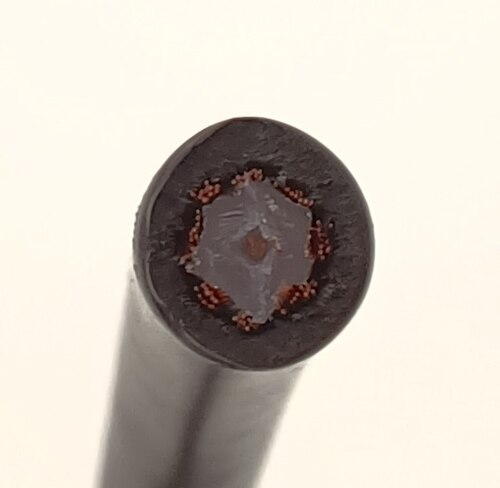
\includegraphics[width=0.46\linewidth]{images/book3/coaxial-cable.jpg}

{\small कोई \omterm{prop:b2:dispersion-wave-packets:coax}{समाक्ष केबल}: भीतरी क्रोड, परावैद्युत, बाहर बुना हुआ चालक --- अर्थात् कोई \omterm{prop:b2:dispersion-wave-packets:coax}{संचरण-रेखा}, जिसकी प्रति मीटर प्रेरकत्व और धारिता उसकी चाल तथा उसकी \omterm{prop:b2:dispersion-wave-packets:coax}{अभिलक्षणिक प्रतिबाधा} तय करती हैं।}
\end{omfigure}

\begin{proposition}[हानिकर रेखा; विरूपण-रहित प्रतिबंध]\label{prop:b2:dispersion-wave-packets:lossy}
\index{हेविसाइड प्रतिबंध}\index{केल्विन का वर्ग-नियम}
प्रति एकांक लंबाई श्रेणी-प्रतिरोध $R$ और पार्श्व-चालकता $G$ लेने पर
समीकरण $\partial_xv = -\Lambda\partial_ti - Ri$, $\partial_xi =
-\Gamma\partial_tv - Gv$ बन जाते हैं, और \omterm{def:b2:dispersion-wave-packets:relation}{परिक्षेपण संबंध} $\underline k^2 = (\Lambda\omega -
\iu R)(\Gamma\omega - \iu G)$: अर्थात् रेखा परिक्षेपी और क्षीणकारी है। दो
सीमाएँ: (क) $R/\Lambda = G/\Gamma$ (हेविसाइड का प्रतिबंध, जो प्रेरकत्व जोड़कर
पाया जाता है): $\underline k = \omega\sqrt{\Lambda\Gamma} - \iu\sqrt{RG}$, अर्थात् हर आवृत्ति
वही चाल और वही \omterm{def:b2:dispersion-wave-packets:complex}{क्षीणन} लेकर चलती है --- रेखा
\emph{क्षीण} तो करती है पर \emph{विरूपित} नहीं। (ख) $\Lambda \approx 0$, $G \approx 0$
(पहली समुद्री केबलें): $\partial_x^2v = R\Gamma\,\partial_tv$, अर्थात् कोई
\emph{विसरण} समीकरण --- तब स्पंद संचरित नहीं होता बल्कि लिप जाता है,
और दूरी $L$ तक $\sim R\Gamma L^2$ समय बाद पहुँचता है (\omterm{prop:b2:dispersion-wave-packets:lossy}{केल्विन का
वर्ग-नियम}), अर्थात् दस गुना लंबी केबल के लिए सौ गुना अधिक समय।
\end{proposition}

\begin{proof}
$\eu^{\iu(\omega t - kx)}$ रखिए: $-\iu kv = -(\iu\omega\Lambda + R)i$, $-\iu ki = -(\iu
\omega\Gamma + G)v$; अब गुणा कीजिए। हेविसाइड के प्रतिबंध पर गुणनफल
पूर्ण वर्ग बन जाता है। विसरण-सीमा $\iu\omega\Lambda$ और $G$ वाले पद छोड़ देती है।
\end{proof}

\begin{example}[तीन केबलें]\label{ex:b2:dispersion-wave-packets:cables}
1858 की अटलांटिक-पार केबल: गटापर्चा में लिपटा एक ही ताँबे का तार,
$R \approx \qty{3}{\ohm/km}$, $\Gamma \approx \qty{0.3}{\micro F/km}$, $L = \qty{3000}{km}$:
$R\Gamma = \qty{9e-10}{s/m^2}$ और प्रति बिंदु $R\Gamma L^2 \approx \qty{8}{s}$: अर्थात् एक शब्द प्रति
मिनट; और संकेत को \qty{2}{kV} से ज़ोर देकर भेजने की चलाने वालों की कोशिशों ने
कुछ ही सप्ताहों में विद्युतरोधन नष्ट कर दिया। हेविसाइड का प्रतिबंध पूरा करने के लिए
प्रति \qty{2}{km} कुंडलियों से भारित कोई दूरभाष-रेखा
(1900): सैकड़ों किलोमीटर तक साफ़ बात। और कोई आधुनिक \qty{50}{\ohm}
\omterm{prop:b2:dispersion-wave-packets:coax}{समाक्ष केबल}: $c = \qty{2e8}{m/s}$, $\Lambda = \qty{0.25}{\micro H/m}$, $\Gamma =
\qty{100}{pF/m}$, और चालकों में त्वचा-प्रभाव के कारण
(\cref{ch:b2:waves-in-media}) $\sqrt f$ की तरह बढ़ता \omterm{def:b2:dispersion-wave-packets:complex}{क्षीणन}: \qty{100}{MHz} पर
प्रति सौ मीटर कुछ \omterm{def:b2:sound-waves:decibel}{डेसिबल}।
\end{example}

\begin{method}[कोई परिक्षेपण संबंध पढ़ना]\label{met:b2:dispersion-wave-packets:method}
(1) माध्यम का \omterm{thm:b2:waves-on-strings:equation}{तरंग-समीकरण} सम्मिश्र संकेतन में लिखिए और
$\underline k(\omega)$ के लिए हल कीजिए। (2) वास्तविक $k$: $v_\varphi = \omega/k$ और
$v_g = \dd\omega/\dd k$ (या $1/(\dd k/\dd\omega)$) निकालिए; और तुलना कीजिए: परिक्षेपी है या नहीं,
सामान्य ($v_g < v_\varphi$) या असामान्य। (3) सम्मिश्र $k$: उसे
संचरण ($k'$) और \omterm{def:b2:dispersion-wave-packets:complex}{क्षीणन} ($k''$, लंबाई $1/k''$) में बाँटिए; शुद्ध
काल्पनिक का अर्थ है क्षयी, कोई परिवहन नहीं। (4) कोई कटाव आवृत्ति
किसी संचरणशील पट्टी को किसी क्षयी पट्टी से अलग करती है। (5) किसी संकेत के लिए
$v_g$ पर चलते आवरण से तर्क कीजिए, शिखरों से कभी नहीं।
\end{method}

\section{अभ्यास}

\begin{exercise}[$\star$]\label{exo:b2:dispersion-wave-packets:1}
\omterm{ex:b2:dispersion-wave-packets:examples}{गहरे पानी की तरंगें}, $\omega^2 = gk$। (क) \qty{100}{m} की किसी स्वेल का \omterm{def:b2:dispersion-wave-packets:relation}{कला वेग}, \omterm{prop:b2:dispersion-wave-packets:group}{समूह वेग} और
आवर्तकाल। (ख) \qty{14}{s} आवर्तकाल की कोई स्वेल:
तरंगदैर्घ्य, $v_\varphi$, $v_g$; और उसकी ऊर्जा को \qty{5000}{km} पार करने में लगा समय।
(ग) \qty{2}{s} आवर्तकाल की छोटी लहरें वहाँ पहुँचती ही क्यों नहीं?
\end{exercise}

\begin{exercise}[$\star$]\label{exo:b2:dispersion-wave-packets:2}
कोई माध्यम $\omega^2 = \omega_c^2 + c^2k^2$ का पालन करता है, जिसमें $\omega_c = 2\pi \times \qty{1e7}{rad/s}$
और $c = \qty{3e8}{m/s}$। $f = \qty{20}{MHz}$ के लिए: $k$, $v_\varphi$, $v_g$, और
उनका गुणनफल। $f = \qty{5}{MHz}$ के लिए: $\kappa$ और वेधन गहराई।
\end{exercise}

\begin{exercise}[$\star$]\label{exo:b2:dispersion-wave-packets:3}
\qty{440}{Hz} और \qty{444}{Hz} के दो स्वरित्र द्विभुज: विस्पंद आवृत्ति, और
प्रबलता के उतार-चढ़ाव का आवर्तकाल। \qty{100}{m} और \qty{110}{m}
तरंगदैर्घ्यों की दो जल-तरंगें: आवृत्तियाँ, आवरण की तरंगदैर्घ्य और
चाल; \qty{105}{m} पर $v_g$ से तुलना कीजिए।
\end{exercise}

\begin{exercise}[$\star$]\label{exo:b2:dispersion-wave-packets:4}
कोई \omterm{prop:b2:dispersion-wave-packets:coax}{समाक्ष केबल}: भीतरी चालक \qty{0.9}{mm} व्यास का, बाहरी
\qty{3.0}{mm}, पॉलिथीन ($\varepsilon_r = 2.3$)। $\Lambda$, $\Gamma$, तरंग-चाल,
\omterm{prop:b2:dispersion-wave-packets:coax}{अभिलक्षणिक प्रतिबाधा}, प्रति मीटर विलंब; और \qty{10}{ns} के विलंब के तुल्य
केबल की लंबाई। वही केबल, पॉलिथीन के बदले हवा के साथ।
\end{exercise}

\begin{exercise}[$\star\star$]\label{exo:b2:dispersion-wave-packets:5}
\emph{कड़ा तार।} कोई वास्तविक पियानो-तार $\mu\partial_t^2y = T\partial_x^2y
- EI\,\partial_x^4y$ का पालन करता है ($EI$ बंकन-दृढ़ता)। (क) \omterm{def:b2:dispersion-wave-packets:relation}{परिक्षेपण संबंध},
कला और \omterm{prop:b2:dispersion-wave-packets:group}{समूह वेग}। (ख) \cref{ch:b2:waves-on-strings} के A$_4$ तार
($T = \qty{685}{N}$, $\mu = \qty{6.1}{g/m}$, $EI =
\qty{9.8e-3}{N.m^2}$) के लिए, $v_\varphi$ की सापेक्ष वृद्धि, आठवें संनादी के
लिए ($k = 8\pi/L$, $L = \qty{0.38}{m}$); और वहाँ मिली असंनादिता से जाँचिए। (ग) परिक्षेपण
सामान्य है या असामान्य? कुछ आवाजाहियों के बाद कोई तीखा छेड़
कैसा दिखता है?
\end{exercise}

\begin{exercise}[$\star\star$]\label{exo:b2:dispersion-wave-packets:6}
\emph{अवमंदित तार।} $\mu\partial_t^2y + \alpha\partial_ty = T\partial_x^2y$। (क)
\omterm{def:b2:dispersion-wave-packets:relation}{परिक्षेपण संबंध} निकालिए। (ख) $\alpha \ll \mu\omega$ के लिए दिखाइए कि $k' \approx \omega/c$ और
$k'' \approx \alpha/2Z$; प्रति मीटर \omterm{def:b2:sound-waves:decibel}{डेसिबल} में \omterm{def:b2:dispersion-wave-packets:complex}{क्षीणन}। (ग) अंक: $\mu =
\qty{5}{g/m}$, $T = \qty{50}{N}$, $\alpha = \qty{0.02}{kg.m^{-1}.s^{-1}}$, $f =
\qty{100}{Hz}$: सन्निकटन जाँचिए और $\delta$ दीजिए। (घ) क्या अवमंदित
तार परिक्षेपी है? $\alpha$ की किस दशा में वह हो जाएगा?
\end{exercise}

\begin{exercise}[$\star\star$]\label{exo:b2:dispersion-wave-packets:7}
\emph{तरंगिकाएँ।} छोटी जल-तरंगों पर \omterm{rem:b2:viscous-flows:capillarity}{पृष्ठ तनाव} राज करता है: $\omega^2 =
\gamma k^3/\rho$ ($\gamma = \qty{0.072}{N/m}$); और पूरा संबंध $\omega^2 = gk +
\gamma k^3/\rho$ है। (क) शुद्ध केशिका तरंगों के लिए $v_\varphi$ और $v_g$; कौन-सा
बड़ा है? (ख) दिखाइए कि पूरे संबंध का \omterm{def:b2:dispersion-wave-packets:relation}{कला वेग}
$\lambda_m = 2\pi\sqrt{\gamma/\rho g}$ पर न्यूनतम है, और $\lambda_m$ तथा $v_{\min}$ निकालिए।
(ग) $v_{\min}$ से धीमी कोई नाव कोई अनुतरंग नहीं बनाती: क्यों? (घ) किसी तालाब पर
वर्षा-बूँदें ऐसे छल्ले बनाती हैं जिनके शिखर छल्ले से पीछे रह जाते हैं: किस दशा में?
\end{exercise}

\begin{exercise}[$\star\star$]\label{exo:b2:dispersion-wave-packets:8}
\emph{फैलाव।} $\Delta x_0$ आरंभिक चौड़ाई का कोई पुंज
$t_{\text{फैलाव}} \approx \Delta x_0^2/|\omega''(k_0)|$ बाद अपनी चौड़ाई दुगुनी कर लेता है। (क) गहरे पानी की
तरंगों का कोई समूह, $\lambda = \qty{50}{m}$, $\Delta x_0 = \qty{500}{m}$। (ख) किसी काँच-तंतु में
प्रकाश का कोई स्पंद: $\omega'' \approx \qty{-0.16}{m^2/s}$; \qty{10}{ps} का स्पंद ($\Delta x_0 =
\qty{2}{mm}$): फैलाव-काल और उतने में तय की गई दूरी; और वही
\qty{1}{ns} के स्पंद के लिए। लंबी प्रकाशिक कड़ियाँ लंबे स्पंद या
परिक्षेपण-प्रतिकारी तंतु क्यों काम में लेती हैं?
\end{exercise}

\begin{exercise}[$\star\star$]\label{exo:b2:dispersion-wave-packets:9}
\emph{समुद्री केबल।} $R = \qty{3}{\ohm/km}$, $\Gamma = \qty{0.3}{\micro F/km}$,
और $\Lambda$ तथा $G$ नगण्य। (क) दिखाइए कि $v$ किसी विसरण समीकरण का पालन करता है और
उसकी विसरणशीलता दीजिए। (ख) \omterm{def:b2:dispersion-wave-packets:relation}{परिक्षेपण संबंध} $\underline k(\omega)$; \qty{1}{Hz} और \qty{10}{Hz} पर \omterm{def:b2:dispersion-wave-packets:relation}{कला
वेग} तथा \omterm{def:b2:dispersion-wave-packets:complex}{क्षीणन} लंबाई। (ग)
\qty{3000}{km} पर किसी संकेत के ``पहुँचने'' का समय ($\sim R\Gamma L^2$); और प्रति
मिनट शब्द। (घ) हेविसाइड का उपचार: $R/\Lambda = G/\Gamma$ के लिए प्रति किलोमीटर
आवश्यक प्रेरकत्व, यदि $G = \qty{1e-7}{S/km}$ हो; उसे जोड़ना कठिन क्यों था?
\end{exercise}

\begin{exercise}[$\star\star\star$]\label{exo:b2:dispersion-wave-packets:10}
\emph{ऊर्जा \omterm{prop:b2:dispersion-wave-packets:group}{समूह वेग} से चलती है।} प्रत्यास्थ शय्या पर तार:
$\mu\partial_t^2y = T\partial_x^2y - Ky$, तरंग $y = A\cos(\omega t - kx)$, जहाँ $\omega^2 =
\omega_c^2 + c^2k^2$। (क) ऊर्जा घनत्व $e = \tfrac12\mu(\partial_ty)^2 + \tfrac12T
(\partial_xy)^2 + \tfrac12Ky^2$ और अभिवाह $\mathcal P = -T\partial_xy\,\partial_ty$:
$\partial_te + \partial_x\mathcal P = 0$ जाँचिए। (ख) तरंग के लिए समय-औसत $\langle e\rangle$ और
$\langle\mathcal P\rangle$। (ग) दिखाइए कि $\langle\mathcal P\rangle/
\langle e\rangle = c^2k/\omega = v_g$ है, $v_\varphi$ नहीं। (घ) कटाव से नीचे
ऊर्जा-अभिवाह का क्या होता है?
\end{exercise}

\begin{exercise}[$\star\star\star$]\label{exo:b2:dispersion-wave-packets:11}
\emph{स्वेल और सुनामी।} $\lambda$ तरंगदैर्घ्य की जल-तरंगें $h$ गहराई पर
$\omega^2 = gk\tanh kh$ का पालन करती हैं (स्वीकृत)। (क) गहरे पानी की और
उथले पानी ($kh \ll 1$) की सीमाएँ फिर से पाइए; उथले पानी की तरंगों की चाल; क्या
वे परिक्षेपी हैं? (ख) \qty{4}{km} गहरे समुद्र पर $\lambda = \qty{200}{km}$ की कोई सुनामी:
कौन-सी सीमा, चाल, आवर्तकाल; और \qty{8000}{km} पार करने में लगा समय। (ग) तट से दूर
उसका आयाम \qty{0.5}{m} है: \qty{1000}{km} के अग्र-भाग के लिए प्रति एकांक लंबाई
शिखर की ऊर्जा (प्रति एकांक क्षेत्रफल $E = \tfrac12\rho gA^2$ स्वीकार कीजिए); और गहराई
\qty{10}{m} रह जाने पर क्या होता है, यदि ऊर्जा-अभिवाह $Ev_g$
संरक्षित रहे (ग्रीन का नियम, $A \propto h^{-1/4}$)? (घ) किसी तट पर आती
\qty{100}{m} की स्वेल: वह किस गहराई पर तल को अनुभव करने लगती है,
और उसके शिखर किनारे के समांतर क्यों मुड़ जाते हैं?
\end{exercise}

\begin{exercise}[$\star\star\star$]\label{exo:b2:dispersion-wave-packets:12}
\emph{रेखा पर कोई स्पंद।} $\ell = \qty{100}{m}$ लंबाई की कोई \qty{50}{\ohm} केबल
($c = \qty{2e8}{m/s}$) $x = 0$ पर \qty{50}{\ohm} आंतरिक प्रतिरोध के जनित्र से
चलाई जाती है और $x = \ell$ पर भार $R_L$ पर समाप्त होती है। (क) दिखाइए
कि सिरे पर पहुँचती कोई तरंग वोल्टता-गुणांक
$r = (R_L - Z_c)/(R_L + Z_c)$ से परावर्तित होती है ($v$ और $i$ को आपतित
तथा परावर्तित तरंगों के योग के रूप में लिखिए और भार में ओम का नियम लगाइए)। (ख)
$R_L = 50$, $0$, $\infty$, \qty{150}{\ohm} के लिए मान। (ग) \qty{1}{V} का \qty{1}{ns} स्पंद
भेजा जाता है: हर भार के लिए जनित्र पर लगा दोलनदर्शी क्या, और कब,
दिखाता है; और जनित्र के \qty{50}{\ohm} क्यों मायने रखते हैं। (घ) किसी दबी हुई
केबल का कोई दोष \qty{1.8}{\micro s} बाद प्रतिध्वनि लौटाता है: वह कहाँ है? (काल-प्रांत
परावर्तनमिति।)
\end{exercise}

\section{समस्या: केबल और समुद्र}

\begin{problem}[{सप्ताहांत समस्या --- परिक्षेपण काम पर: वह तार-केबल
जिसने बिंदुओं को लीप दिया, वह स्वेल जो तूफ़ान की सूचना देती है, वह
सुनामी जो पूरा महासागर पार कर जाती है, और वह पुंज जो फैलता है}]
\label{pb:b2:dispersion-wave-packets:1}

\medskip
\noindent\textbf{भाग I --- तार-केबल।}
1866 की अटलांटिक-पार केबल: $R = \qty{2.0}{\ohm/km}$, $\Gamma = \qty{0.25}{\micro F/km}$,
$\Lambda = \qty{0.5}{mH/km}$, $G$ नगण्य, लंबाई $L = \qty{3500}{km}$।
\begin{enumerate}
  \item $R$ के साथ \omterm{prop:b2:dispersion-wave-packets:coax}{टेलीग्राफ समीकरण} लिखिए और
        \omterm{def:b2:dispersion-wave-packets:relation}{परिक्षेपण संबंध} $\underline k^2 = \Gamma\omega(\Lambda\omega - \iu R)$ निकालिए।
  \item किस आवृत्ति पर $\Lambda\omega$ $R$ के बराबर होता है? इससे निष्कर्ष निकालिए कि
        तार-संचार की आवृत्तियों (कुछ हर्ट्ज़) पर रेखा
        विसरणशील दशा में है।
  \item उस दशा में $\underline k = \sqrt{-\iu R\Gamma\omega}$: $k'$ और $k''$ दीजिए
        (याद रखिए $\sqrt{-\iu} = (1 - \iu)/\sqrt2$); \qty{1}{Hz} पर और \qty{4}{Hz} पर
        \omterm{def:b2:dispersion-wave-packets:relation}{कला वेग} तथा \omterm{def:b2:dispersion-wave-packets:complex}{क्षीणन} लंबाई।
  \item \qty{1}{Hz} पर और \qty{4}{Hz} पर पूरी केबल पर \omterm{def:b2:sound-waves:decibel}{डेसिबल} में \omterm{def:b2:dispersion-wave-packets:complex}{क्षीणन}।
        कौन-सी आवृत्ति बची रहती है? इससे किसी तीखे बिंदु का
        क्या होता है?
  \item केल्विन का पारगमन-काल का आकलन, $R\Gamma L^2$; और यदि कोई शब्द लगभग
        $10$ बिंदुओं-रेखाओं का हो तथा बिंदु अतिव्यापी न हों, तो
        केबल की प्रति मिनट शब्दों में व्यावहारिक दर।
  \item हेविसाइड ने $\Lambda$ बढ़ाने का सुझाव दिया: किस मान पर \qty{4}{Hz} पर
        $\Lambda\omega = R$ होता है, और तब चाल तथा \omterm{def:b2:dispersion-wave-packets:complex}{क्षीणन} क्या होते
        ($G = 0$ लीजिए, अतः प्रतिबंध $R/\Lambda = G/\Gamma$ ठीक-ठीक पूरा नहीं
        हो सकता --- उस आवृत्ति पर सामान्य संबंध काम में लीजिए)?
  \item कोई आधुनिक प्रकाशिक तंतु \qty{1e10}{bit/s} ढोता है:
        प्रश्न 5 से दस की घातों में तुलना कीजिए।
\end{enumerate}

\medskip
\noindent\textbf{भाग II --- स्वेल।}
गहरा पानी: $\omega^2 = gk$।
\begin{enumerate}[resume]
  \item आवर्तकाल $T$ के फलन के रूप में कला और \omterm{prop:b2:dispersion-wave-packets:group}{समूह वेग}।
  \item किसी तट से \qty{4000}{km} दूर कोई तूफ़ान \qty{6}{s} से \qty{18}{s} तक के
        आवर्तकालों की तरंगें बनाता है: दोनों छोरों का पहुँचने का समय;
        और स्वेल-घटना की अवधि।
  \item दिखाइए कि $D$ दूरी के किसी तट पर आता आवर्तकाल
        $1/T = gt/4\pi D$ का पालन करता है, जहाँ $t$ तूफ़ान से गिना गया है: अर्थात् $1/T$
        समय में रैखिक रूप से बढ़ता है। कोई प्लव किसी दिन दोपहर $T = \qty{16}{s}$
        लिखता है और ठीक \qty{24}{h} बाद $T = \qty{12}{s}$: तूफ़ान की
        दूरी।
  \item $A$ आयाम की किसी स्वेल की प्रति एकांक क्षेत्रफल ऊर्जा $\tfrac12\rho
        gA^2$ है; \qty{1}{m} शिखर की रेखा को पार करती शक्ति, $A =
        \qty{1.5}{m}$, $T = \qty{12}{s}$ के लिए। (\omterm{prop:b2:dispersion-wave-packets:group}{समूह वेग} लीजिए --- क्यों?)
  \item \qty{1}{km} अग्र-भाग का कोई तरंग-ऊर्जा फ़ार्म, $30\%$ दक्षता के साथ:
        वैद्युत शक्ति; किसी पवन-चक्की (\qty{3}{MW}) से तुलना कीजिए।
  \item गहरे पानी पर \qty{5}{m/s} से चलती कोई नाव अपने पीछे कोई अचल
        अनुतरंग छोड़ती है: किस तरंगदैर्घ्य का \omterm{def:b2:dispersion-wave-packets:relation}{कला वेग}
        नाव की चाल के बराबर है और इसलिए उसके साथ चलता है? और आकृति किसी V में
        क्यों घिसटती है, जो शिखरों के अपने फैलाव से सोची जाने वाली चौड़ाई से
        सँकरी है (सोचिए $v_g = v_\varphi/2$)?
  \item किसी चट्टान से स्वेल के एक समूह को देखते हुए बताइए कि समूह के
        किसी स्थिर प्लव से गुज़रने के दौरान कोई एक शिखर क्या करता है;
        $T = \qty{12}{s}$ पर \qty{2}{min} अवधि के समूह में कितने
        शिखर होते हैं, और वह कितनी शिखर-``आयुओं'' के
        बराबर है?
\end{enumerate}

\medskip
\noindent\textbf{भाग III --- सुनामी।}
$\omega^2 = gk\tanh kh$; प्रशांत महासागर की गहराई $h = \qty{4.0}{km}$।
\begin{enumerate}[resume]
  \item कोई भूकंप समुद्र-तल के \qty{100}{km} के टुकड़े को \qty{2}{m} उठा देता है;
        तरंग की $\lambda \approx \qty{200}{km}$ है: जाँचिए कि वह उथले पानी की
        तरंग है और उसकी चाल, आवर्तकाल तथा \qty{6000}{km} दूर के
        तट तक पहुँचने का समय दीजिए।
  \item क्या वह परिक्षेपी है? भाग II की स्वेल से तुलना कीजिए: क्या वह
        स्वेल से पहले पहुँचती है या बाद में? कौन-सी एक ही
        स्पंद के रूप में आती है?
  \item तट से दूर उसकी ऊँचाई \qty{0.6}{m} है: प्रति वर्ग मीटर ऊर्जा;
        \qty{500}{km} लंबे अग्र-भाग की एक तरंगदैर्घ्य पर फैली कुल
        ऊर्जा; किसी \qty{1}{Mt} विस्फोट (\qty{4.2e15}{J}) से तुलना कीजिए।
  \item ग्रीन का नियम: तट के पास गहराई \qty{20}{m} रह जाने पर ऊँचाई
        (ऊर्जा-अभिवाह $\tfrac12\rho gA^2v_g$ संरक्षित, $v_g = \sqrt{gh}$);
        वहाँ चाल और तरंगदैर्घ्य; और तरंग तब खड़ी होकर किसी दीवार की तरह
        क्यों टूटती है।
  \item समुद्र में कोई जहाज़ गुज़रती सुनामी को भाँप तक नहीं पाता: क्यों?
  \item \qty{6000}{km} दूर लगे ज्वार-मापी तरंग को लिखते हैं: यात्रा-काल से
        क्या मिलता है, और बदलती गहराई के महासागर पर नापी गई चाल
        $\sqrt{gh}$ से कुछ कम क्यों निकलती है।
\end{enumerate}

\medskip
\noindent\textbf{भाग IV --- फैलता पुंज।}
\begin{enumerate}[resume]
  \item गहरे पानी के लिए $\omega''(k) = \dd^2\omega/\dd k^2$ निकालिए और
        $\lambda = \qty{100}{m}$ के लिए उसका मान।
  \item ऐसी \qty{10}{} तरंगों का कोई पुंज ($\Delta x_0 \approx \qty{1}{km}$)
        छोड़ा जाता है: फैलाव-काल $\Delta x_0^2/|\omega''|$; और उतने में पुंज की
        तय की गई दूरी।
  \item शब्दों में समझाइए कि सँकरे वर्णक्रम वाला (अर्थात् लंबी रेल वाला)
        पुंज धीरे क्यों फैलता है, और भाग III की सुनामी
        लगभग बिलकुल क्यों नहीं फैलती।
  \item वही आकलन किसी ऐसे इलेक्ट्रॉन के लिए, जिसकी तरंगदैर्घ्य \qty{0.1}{nm} है
        और जो \qty{1}{nm} के भीतर स्थानीकृत है, तथा $\omega = \hbar k^2/2m$ ($\hbar =
        \qty{1.05e-34}{J.s}$, $m = \qty{9.1e-31}{kg}$): फैलाव-काल और
        तय की गई दूरी --- अर्थात् \cref{ch:b2:schrodinger-wave-functions} के
        क्वांटम \omterm{prop:b2:dispersion-wave-packets:group}{तरंग-पुंज} से पहली भेंट।
  \item एक सारणी में सार दीजिए: केबल, स्वेल, सुनामी और
        इलेक्ट्रॉन के लिए \omterm{def:b2:dispersion-wave-packets:relation}{परिक्षेपण संबंध}, $v_\varphi$, $v_g$, और
        यह कि माध्यम फैलाता है या केवल क्षीण करता है।
\end{enumerate}
\end{problem}
